\section{Appendix}\label{sec:Appendix}

\paragraph{Servlet Lifecycle}
Figure~\ref{fig:Server_Servlet} describes the complete lifecycle of a servlet w.r.t. a web server and a web container. The lifecycle steps are described as follows \cite{servlet}:

\begin{figure}[h]
	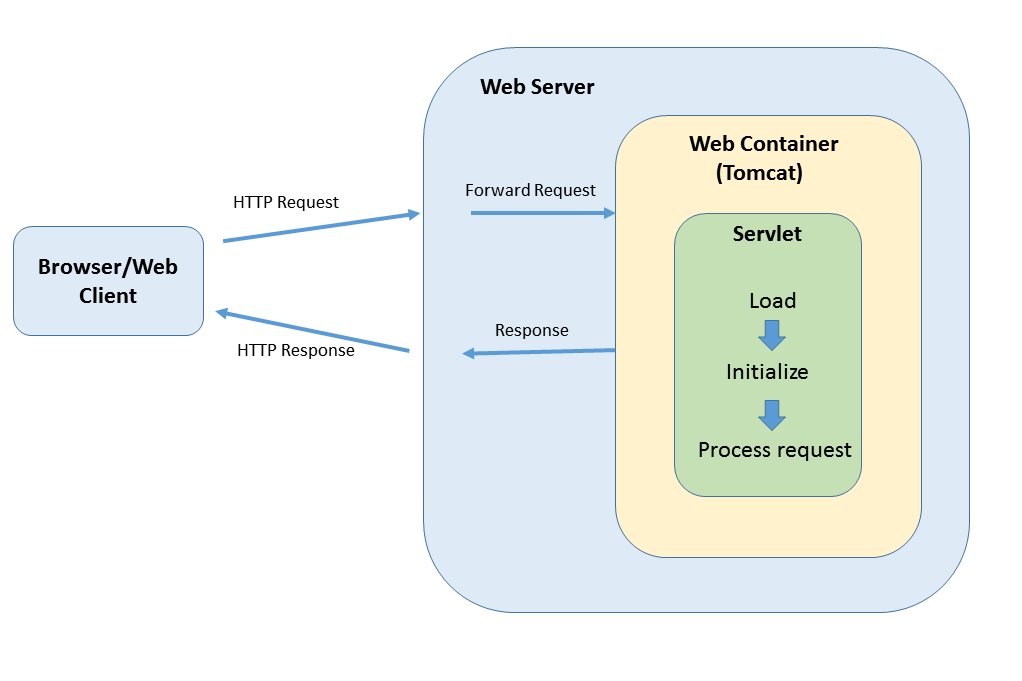
\includegraphics[width=1\textwidth]{figures/Server_Servlet}
	\caption{Servlet Lifecycle}
	\label{fig:Server_Servlet}
\end{figure}

\begin{enumerate}
	\item {The web server receives the \texttt{HTTP request} from the client interacting through a browser.}
	\item {After accepting the request, web server forwards the request to the web container i.e., tomcat.}
	\item {Web container sends the request to the \texttt{Servlet class}.}
	\item {If an instance of the servlet does not exist, the web container}\\\\
	loads the servlet class then creates an instance of the servlet class and initializes the servlet instance by calling the \texttt{init} method.
	\item {After that, web container invokes the \texttt{service} methods (normally HTTP methods i.e., \texttt{get} , \texttt{post} , \texttt{put} , \texttt{delete}) of the servlet class by passing the request and response objects and the actual processing of the request is done and the response is generated.}
	\item {Web container sends the response to the web server. Afterward, web server creates the HTTP response and send it back to the client.}
\end{enumerate}

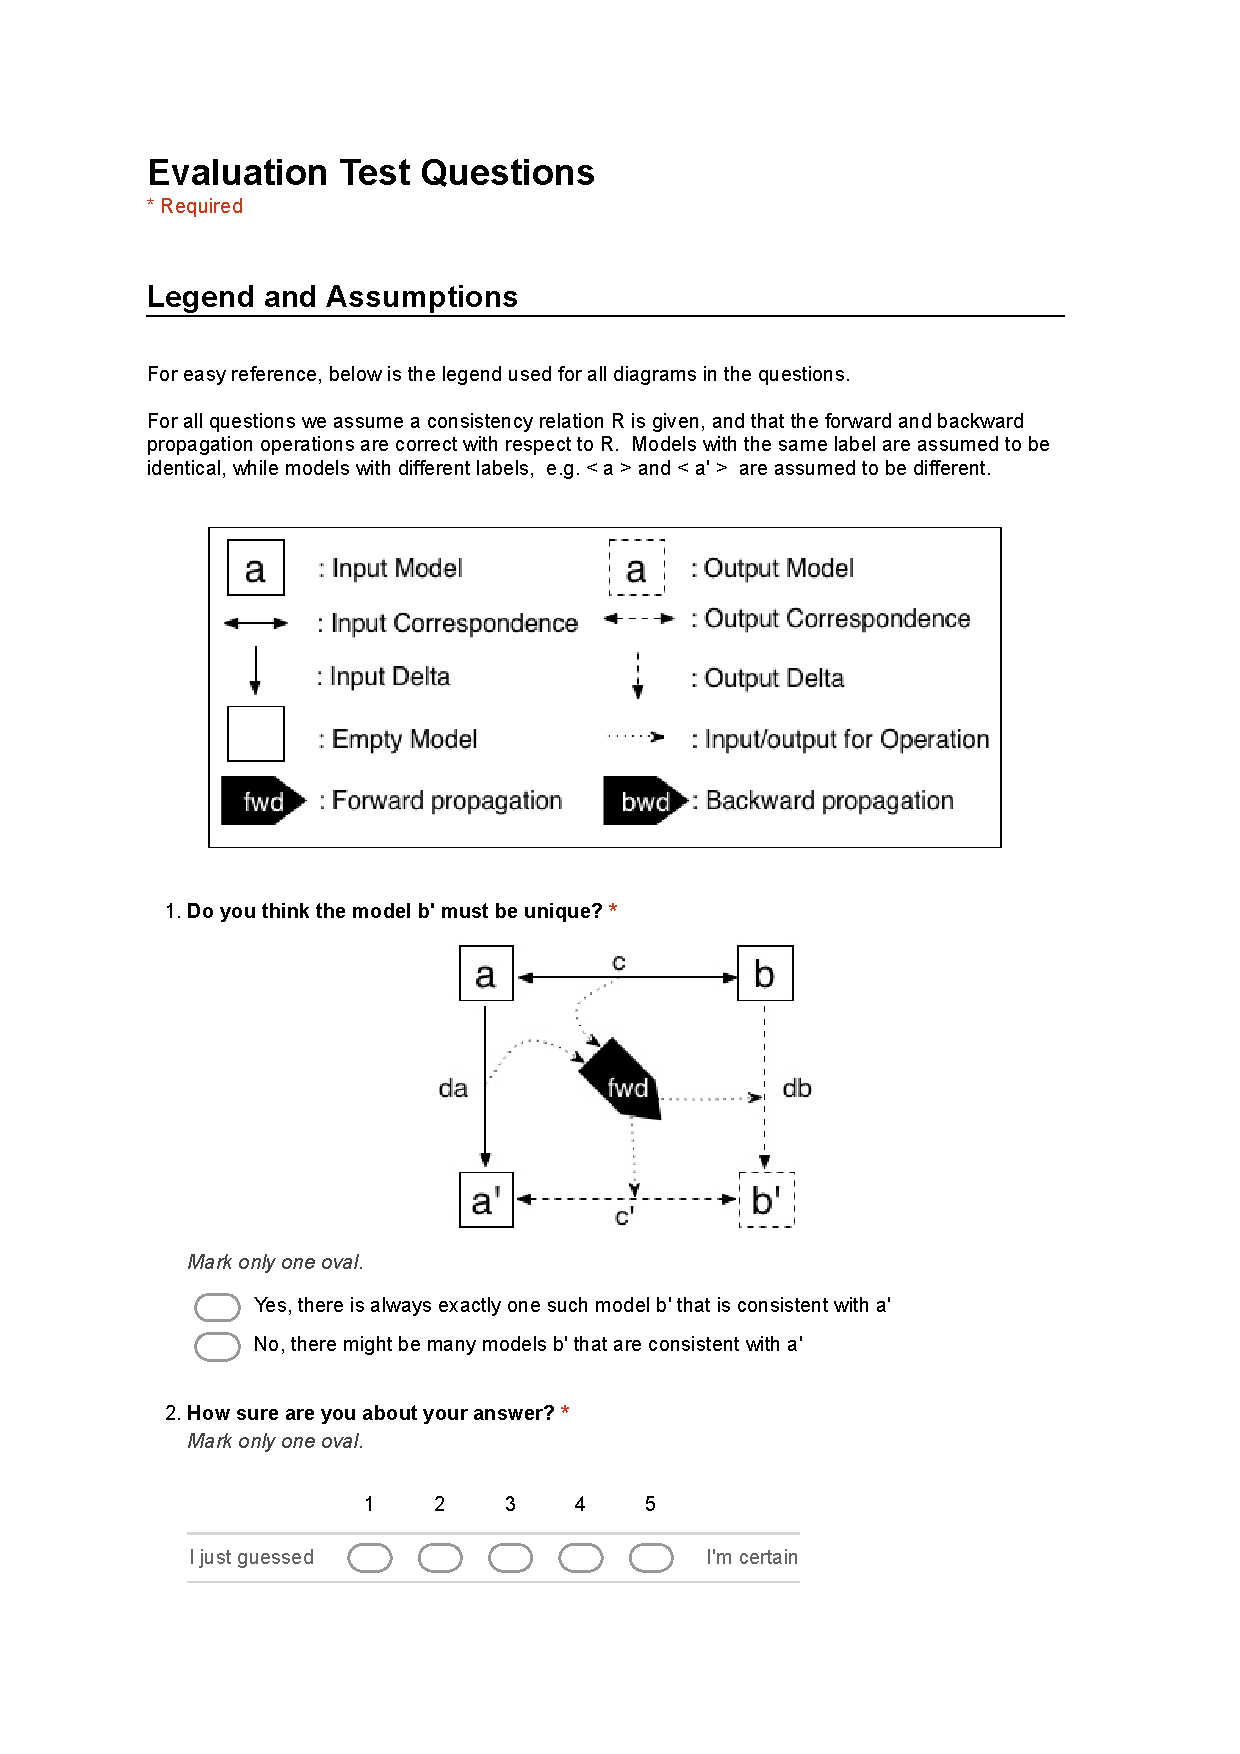
\includepdf[pages={1-4}]{figures/Evaluation_TestQuestions}

